\begin{figure}[t]
  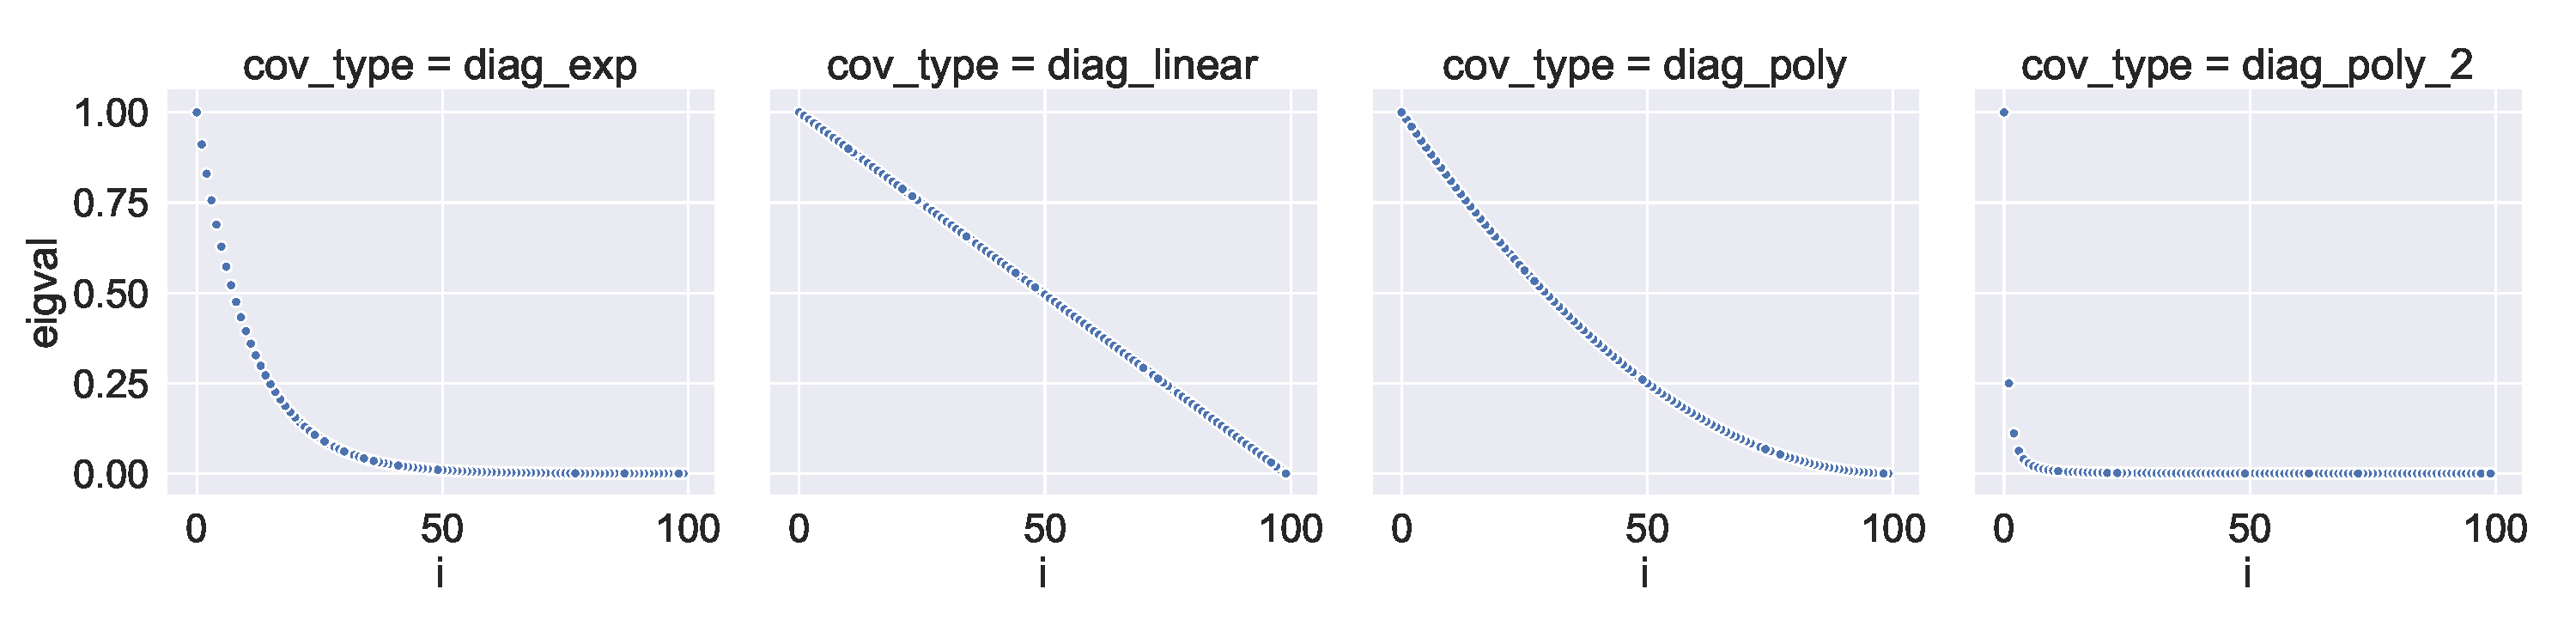
\includegraphics[width=\textwidth]{continuous_figures/decays.pdf}
  \vspace{-1cm}
  \caption{Scree-plots of $\Sigmab$ for the eigenvalue decays examined
    in our empirical valuations. Here $d=100$ for visualization, whereas
    our experiments increase $d$ while preserving the ratio $n/d$ and
    the decay profile,
    with $\lambda_{\text{max}}(\Sigmab) = 1$ to
    $\lambda_{\text{min}}(\Sigmab) = 10^{-4}$.}
  \label{fig:eig-decays}
\end{figure}

% Denoting
% $\lambda_1,...,\lambda_d$ as the eigenvalues of $\Sigmab$, w
Letting $\lambda_i(\Sigmab)$ be the $i$th largest eigenvalue of
$\Sigmab$, we consider the
following eigenvalue profiles:
\begin{itemize}
  \item \texttt{diag\_linear}: linear decay, $\lambda_i(\Sigmab)= b-a i$;
  \item \texttt{diag\_exp}: exponential decay, $\lambda_i(\Sigmab) = b\,10^{- a i} $;
  \item \texttt{diag\_poly}: fixed-degree polynomial decay, $\lambda_i(\Sigmab) = (b-a i)^2$;
  \item \texttt{diag\_poly\_2}: variable-degree polynomial decay, $\lambda_i(\Sigmab) = b i^{-a}$.
\end{itemize}
The constants $a$ and $b$ are chosen to ensure $\lambda_{\text{max}}(\Sigmab) = 1$ and
$\lambda_{\text{min}}(\Sigmab) = 10^{-4}$ (i.e., the condition number
$\kappa(\Sigmab) = 10^{4}$ remains constant).




We verify our conjectures by increasing $d$ while keeping the aspect ratio
$n/d$ fixed and examining the rate of decay of the quantities asserted
in the conjectures. As no closed form expressions are available for
the expectations in the conjectures, we estimate $\E\big[\tr(\W^\dagger)\big]$ (for
Conjecture~\ref{c:wishart}) and $\E[\I-\X^\dagger\X]$ (for
Conjecture~\ref{c:projection}) through Monte Carlo sampling. To ensure that
estimation noise is sufficiently small, we continually increase the number
of Monte Carlo samples until the bootstrap confidence intervals are
within $\pm 12.5\%$ of the quantities in \eqref{eq:wishart} and
\eqref{eq:projection}. We found that while
Conjecture~\ref{c:wishart} required a relatively small number of
trials (up to one thousand),
estimation noise was much larger in Conjecture~\ref{c:projection} and
necessitated over two million trials to obtain good estimates
near $d=100$.

% For Conjecture~\ref{c:wishart}, sampling $\W\sim\Pc\Wc(\Sigmab,n)$ is
% elementary and the only nontrivial aspect of computing $\Vc(\Sigmab, n)$
% is solving for $\lambda_n$ such that
% $n = \tr(\Sigmab(\Sigmab + \lambda_n \I)^{-1})$. But notice that
% if we let $\tau_i > 0$ be the eigenvalues of $\Sigmab \succ 0$,
% then
% \begin{align*}
%   \tr(\Sigmab(\Sigmab + \lambda \I)^{-1})
%   &= \sum_{i=1}^d \frac{\tau_i}{\tau_i + \lambda}
% \end{align*}
% which is equal to $d > n$ when $\lambda = 0$ and monotonically decreasing in
% $\lambda$. Hence, $\lambda_n$ is unique and can be found using bisection.

\begin{figure}[ht]
  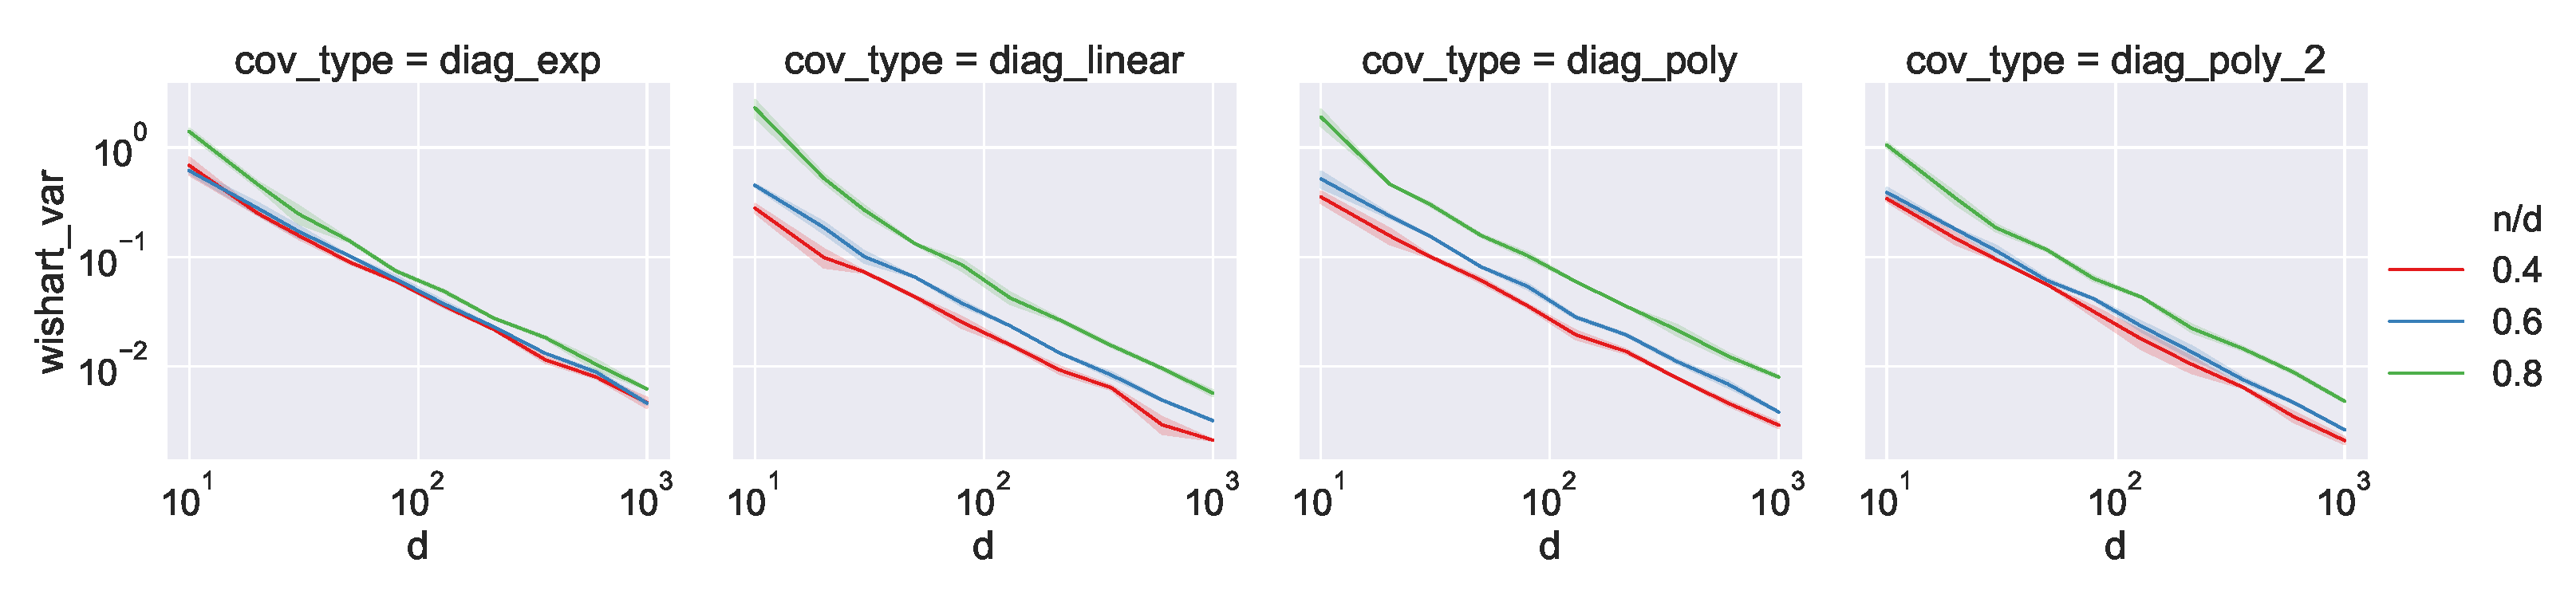
\includegraphics[width=\textwidth]{continuous_figures/wishart_var.pdf}
  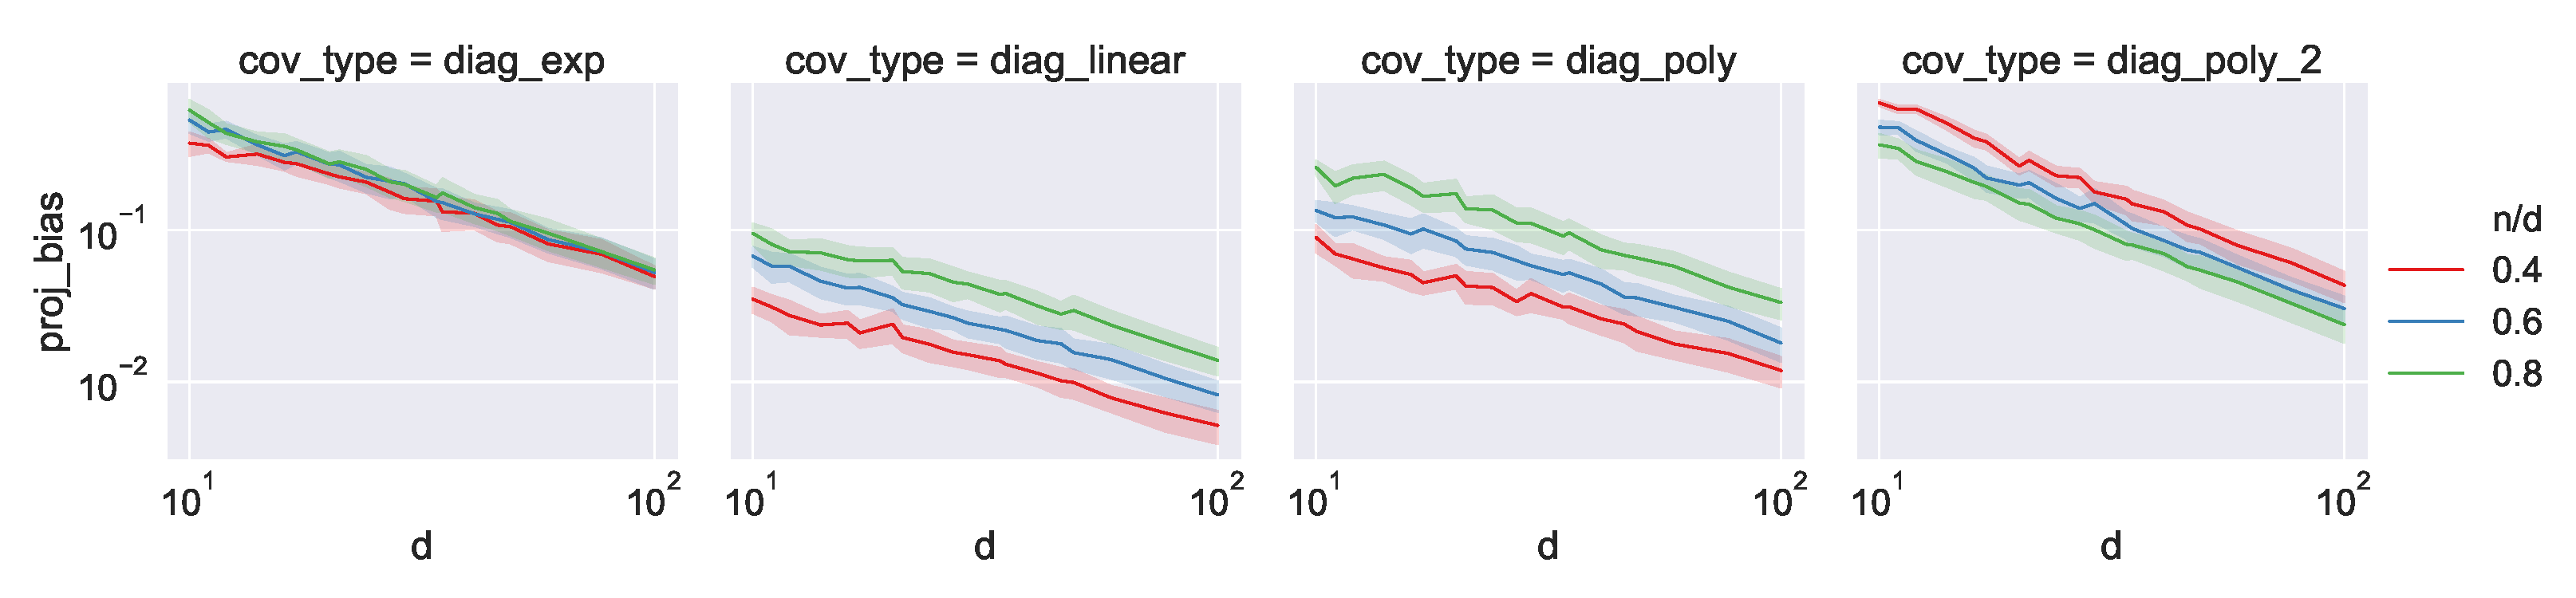
\includegraphics[width=\textwidth]{continuous_figures/proj_bias.pdf}
  \vspace{-1cm}
  \caption{
    Empirical verification of Conjectures~\ref{c:wishart} (top) and
    \ref{c:projection} (bottom).
    We show the quantities
    $|\E[\tr(\W^\dagger)]\,\Vc(\Sigmab,n)^{-1} -1|$ and
    $\|\E[\I-\X^\dagger\X]\Bc(\Sigmab,n)^{-1} - \I\|$, respectively,
    as $d$ increases for various aspect ratios $n/d$.
    Consistent with our conjectures,
    a $O(1/d)$ decay (linear with slope $-1$ on a log-log plot) is
    exhibited across all eigenvalue decay profiles and
    aspect ratios investigated.
  }
  \label{f:conj-wishart}
\end{figure}


The results of empirically validating Conjecture~\ref{c:wishart} are
illustrated in Figure~\ref{f:conj-wishart} (top), where we performed
Monte Carlo estimation of $\E\big[\tr(\W^\dagger)\big]$ and
plot $\big|\E[\tr(\W^\dagger)]\,\Vc(\Sigmab,n)^{-1} -1\big|$
as $d$ increases from $10$ to $1000$, across a range of aspect ratios $n/d$ and eigenvalue
decay profiles for $\Sigmab$. Confidence intervals are estimated by
bootstrapping. We observe that on log-log axes all of the plots are decreasing with
a linear $-1$ slope, consistent with the $O(1/d)$ rate predicted
by Conjecture~\ref{c:wishart}.


Conjecture \ref{c:projection} is handled similarly, by sampling
$\X\sim\mu^n$ where $\mu=\Nc(\zero,\Sigmab )$ to obtain a Monte Carlo estimate of
$\E[\I-\X^\dagger\X]$. To handle the supremum over $\w$, notice that
we can rewrite \eqref{eq:projection} as a spectral norm
\begin{align}
  \sup_{\w\in\R^d\backslash\{\zero\}}\bigg|\frac{\w^\top\E[\I-\X^\dagger\X]\w}{\w^\top
  \Bc(\Sigmab,n)\w} - 1\bigg|
\  =\ \big\|\E[\I-\X^\dagger\X]\Bc(\Sigmab,n)^{-1}
  - \I\big\|.
  \label{eq:proj-to-operator-norm}
\end{align}
Confidence intervals can now be constructed
using existing methods for constructing operator norm
confidence intervals, and our results use the bootstrapping
method described by \cite{lopes2019bootstrapping}.

Figure~\ref{f:conj-wishart} (bottom) shows
how $\big\|\E[\I-\X^\dagger\X]\Bc(\Sigmab,n)^{-1} - \I\big\|$ decays as we
hold the aspect ratio $n/d$ fixed and increase $d$ between $10$ and
$100$ across the listed
eigenvalue decay profiles and aspect ratios. Again, we observe on
log-log axes a linear decay with slope $-1$ consistent with the $O(1/d)$
rate posed by Conjecture~\ref{c:projection}. Note that the range of
$d$ is smaller than in Figure \ref{f:conj-wishart} (top) because the large
number of Monte Carlo samples (up to two million) required for this
experiment made the computations much more expensive.

